\documentclass[compress]{beamer}
\usetheme{sthlm}

%-=-=-=-=-=-=-=-=-=-=-=-=-=-=-=-=-=-=-=-=-=-=-=-=
%        LOADING BEAMER PACKAGES
%-=-=-=-=-=-=-=-=-=-=-=-=-=-=-=-=-=-=-=-=-=-=-=-=

\usepackage{
booktabs,
datetime,
dtk-logos,
graphicx,
multicol,
pgfplots,
ragged2e,
tabularx,
tikz,
wasysym,
multirow,
float,
caption,
subcaption
}

\pgfplotsset{compat=1.8}

\usepackage[utf8]{inputenc}
\usepackage[portuguese]{babel}
\usepackage[T1]{fontenc}
\usepackage{newpxtext,newpxmath}
\usepackage{listings}

\lstset{ %
language=[LaTeX]TeX,
basicstyle=\normalsize\ttfamily,
keywordstyle=,
numbers=left,
numberstyle=\tiny\ttfamily,
stepnumber=1,
showspaces=false,
showstringspaces=false,
showtabs=false,
breaklines=true,
frame=tb,
framerule=0.5pt,
tabsize=4,
framexleftmargin=0.5em,
framexrightmargin=0.5em,
xleftmargin=0.5em,
xrightmargin=0.5em
}



%-=-=-=-=-=-=-=-=-=-=-=-=-=-=-=-=-=-=-=-=-=-=-=-=
%        LOADING TIKZ LIBRARIES
%-=-=-=-=-=-=-=-=-=-=-=-=-=-=-=-=-=-=-=-=-=-=-=-=

\usetikzlibrary{
backgrounds,
mindmap
}

%-=-=-=-=-=-=-=-=-=-=-=-=-=-=-=-=-=-=-=-=-=-=-=-=
%        BEAMER OPTIONS
%-=-=-=-=-=-=-=-=-=-=-=-=-=-=-=-=-=-=-=-=-=-=-=-=

\setbeameroption{show notes}

%-=-=-=-=-=-=-=-=-=-=-=-=-=-=-=-=-=-=-=-=-=-=-=-=
%        BEAMER COMMANDS
%-=-=-=-=-=-=-=-=-=-=-=-=-=-=-=-=-=-=-=-=-=-=-=-=


%-=-=-=-=-=-=-=-=-=-=-=-=-=-=-=-=-=-=-=-=-=-=-=-=
%
%	PRESENTATION INFORMATION
%
%-=-=-=-=-=-=-=-=-=-=-=-=-=-=-=-=-=-=-=-=-=-=-=-=

\title{Arquiteturas distribuídas \\ Parte 02}
\subtitle{DCE540 - Computação Paralela e Distribuída}
%\date{\small{\jobname}}
\author{\texttt{Iago Carvalho}}
\institute{\texttt{Departamento de Ciência da Computação}}

\hypersetup{
pdfauthor = {Iago A. Carvalho},      
pdfsubject = {Computação Paralela e Distribuída},
pdfkeywords = {},  
pdfmoddate= {D:\pdfdate},          
pdfcreator = {WriteLaTeX}
}

\begin{document}

\begin{frame}
\titlepage

\end{frame}

%% --------------------------------------------------------

\begin{frame}{Organização de middleware}

Como vimos na última aula, existem diversas arquiteturas de software
\begin{itemize}
    \item Baseadas em camadas
    \item Baseadas em objetos
    \item Baseadas em recursos
    \item Baseadas em eventos
\end{itemize}

Todas elas são baseadas em \textit{middlewares}

Independente da arquitetura de software desenvolvida, um \textit{middleware} deve implementar dois diferentes \textit{design patterns}
\begin{itemize}
    \item \textit{Wrapper} 
    \item \textit{Interceptor}
\end{itemize}
\end{frame}


%% --------------------------------------------------------

\begin{frame}{\textit{Wrappers}}

Um \textit{wrapper} (ou adaptador) é um \textit{design pattern} que oferece
\begin{itemize}
    \item Interface de comunicação entre componentes
    \item Facilidade de acesso a componentes legados
\end{itemize}

\vspace{0.5cm}

Novamente, existe um paralelo muito grande com Engenharia/Desenvolvimento de softwares

\vspace{0.5cm}

Existem duas formas de se implementar \textit{wrappers}
\begin{itemize}
    \item Na interface de cada componente
    \item Um componente \textit{wrapper}
\end{itemize}

\end{frame}

%% --------------------------------------------------------

\begin{frame}{\textit{Wrappers}}

\centering 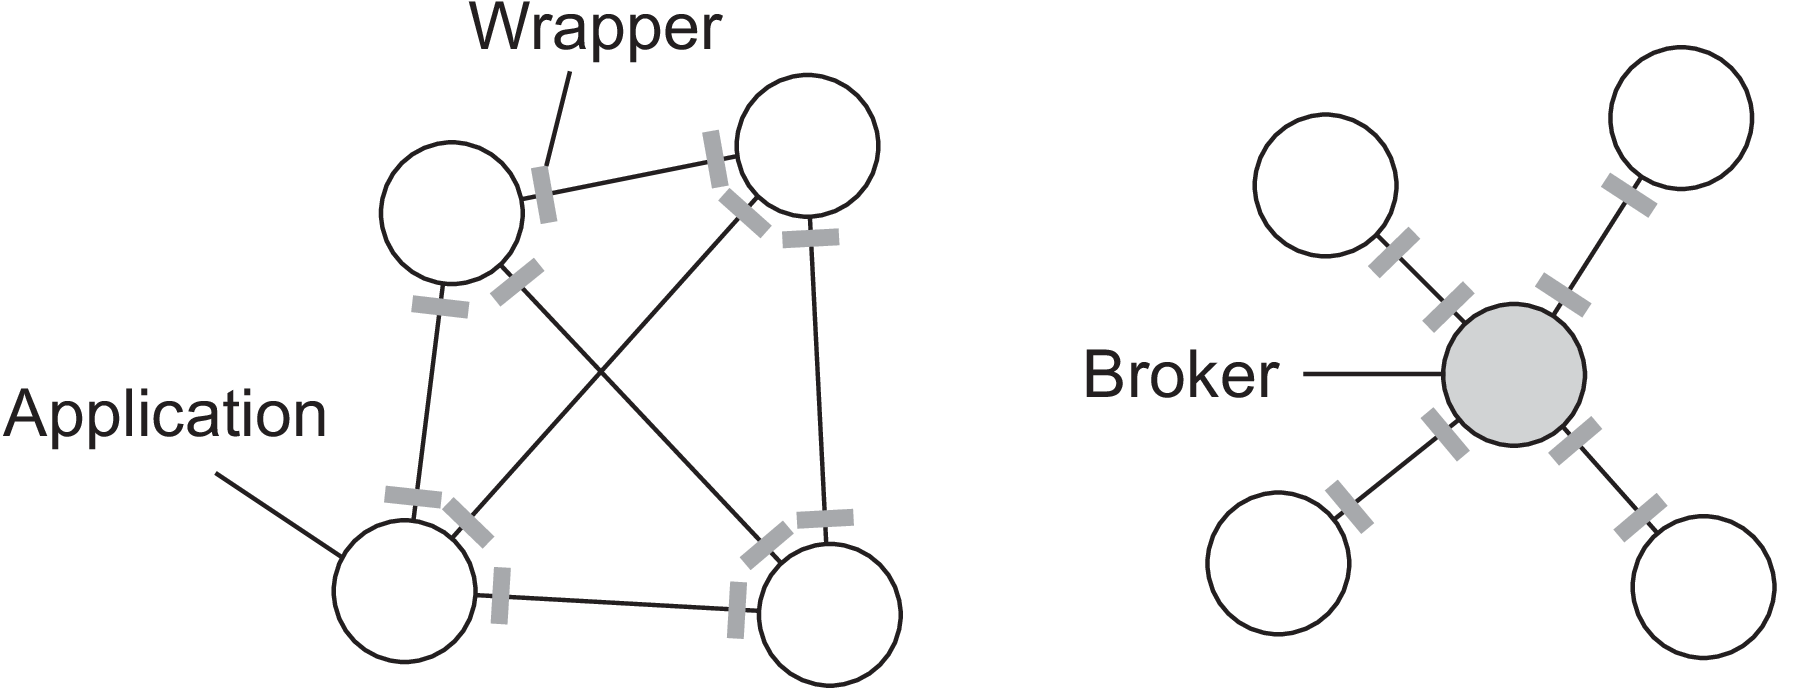
\includegraphics[width=\textwidth]{images/wrappers.png}

\end{frame}

%% --------------------------------------------------------

\begin{frame}{\textit{Interceptor}}

Similar a um \textit{Interrupt handler} de um sistema operacional
\begin{itemize}
    \item Recebe uma requisição
    \item Interrompe o fluxo normal da aplicação
    \item Trata a requisição
    \item Retoma o fluxo normal da aplicação
\end{itemize}

Responsável por fazer a invocação de objetos remotos
\begin{itemize}
    \item Um componente utiliza um método de outro
    \item Componentes localizados em nós diferentes
    \item Localização de cada componente é transparente
    \begin{itemize}
        \item O \textit{interceptor} é responsável por esta transparência
    \end{itemize}
\end{itemize}
\end{frame}

%% --------------------------------------------------------

\begin{frame}{Arquitetura de sistema}

Na aula passada, nós já estudamos arquitetura de software
\begin{itemize}
    \item Como aplicações estão organizadas
    \item Conectores
    \item Interfaces
    \item Componentes
\end{itemize}

Além da arquitetura de software, também é importante falar sobre a arquitetura de sistema
\begin{itemize}
    \item Onde cada software (ou aplicação) está localizado
    \item Como será a iteração entre cada componente
\end{itemize}

Centralizada, distribuída ou híbrida

\end{frame}

%% --------------------------------------------------------

\begin{frame}{Arquitetura de sistema centralizada}

 
É a maneira mais simples de pensarmos
\begin{itemize}
    \item Cliente-servidor
    \item Uma ou mais camadas
    \item Protocolo orientado a conexão ou não
    \begin{itemize}
        \item Exemplo: TCP e UDP
    \end{itemize}
\end{itemize}
    
\vspace{1cm}

\centering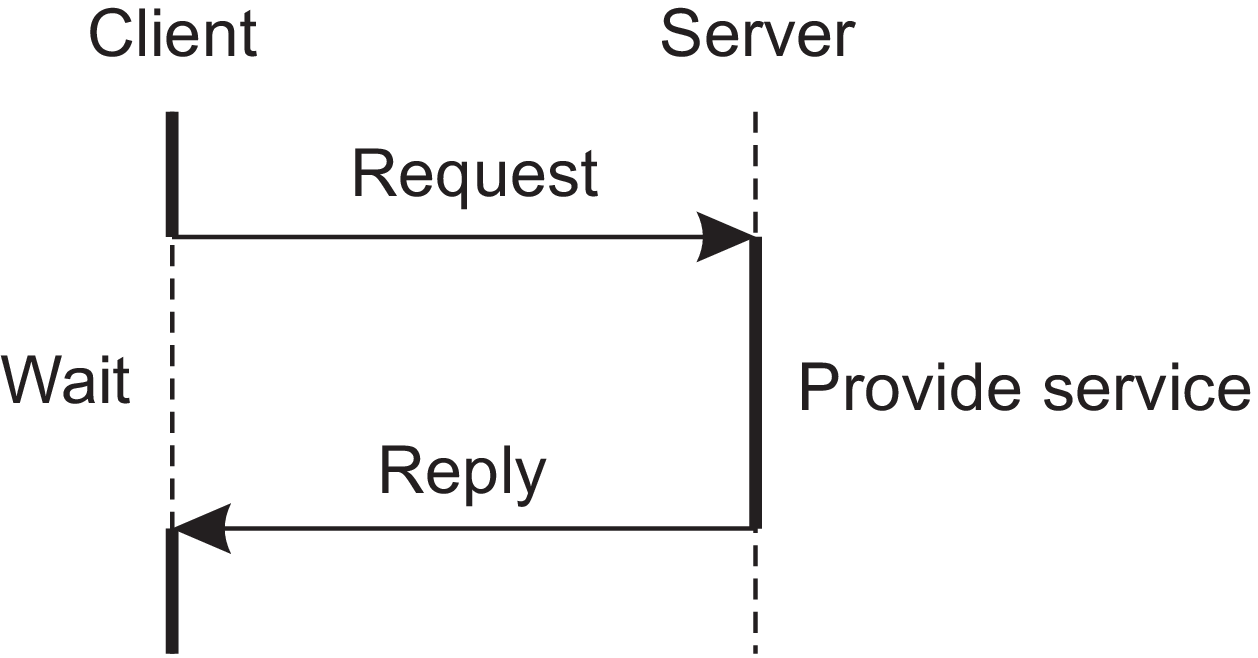
\includegraphics[width=0.65\linewidth]{images/client-server.png}

\end{frame}

%% --------------------------------------------------------

\begin{frame}{Arquitetura de sistema centralizada multi-camadas}

\vspace{1cm}
 
\centering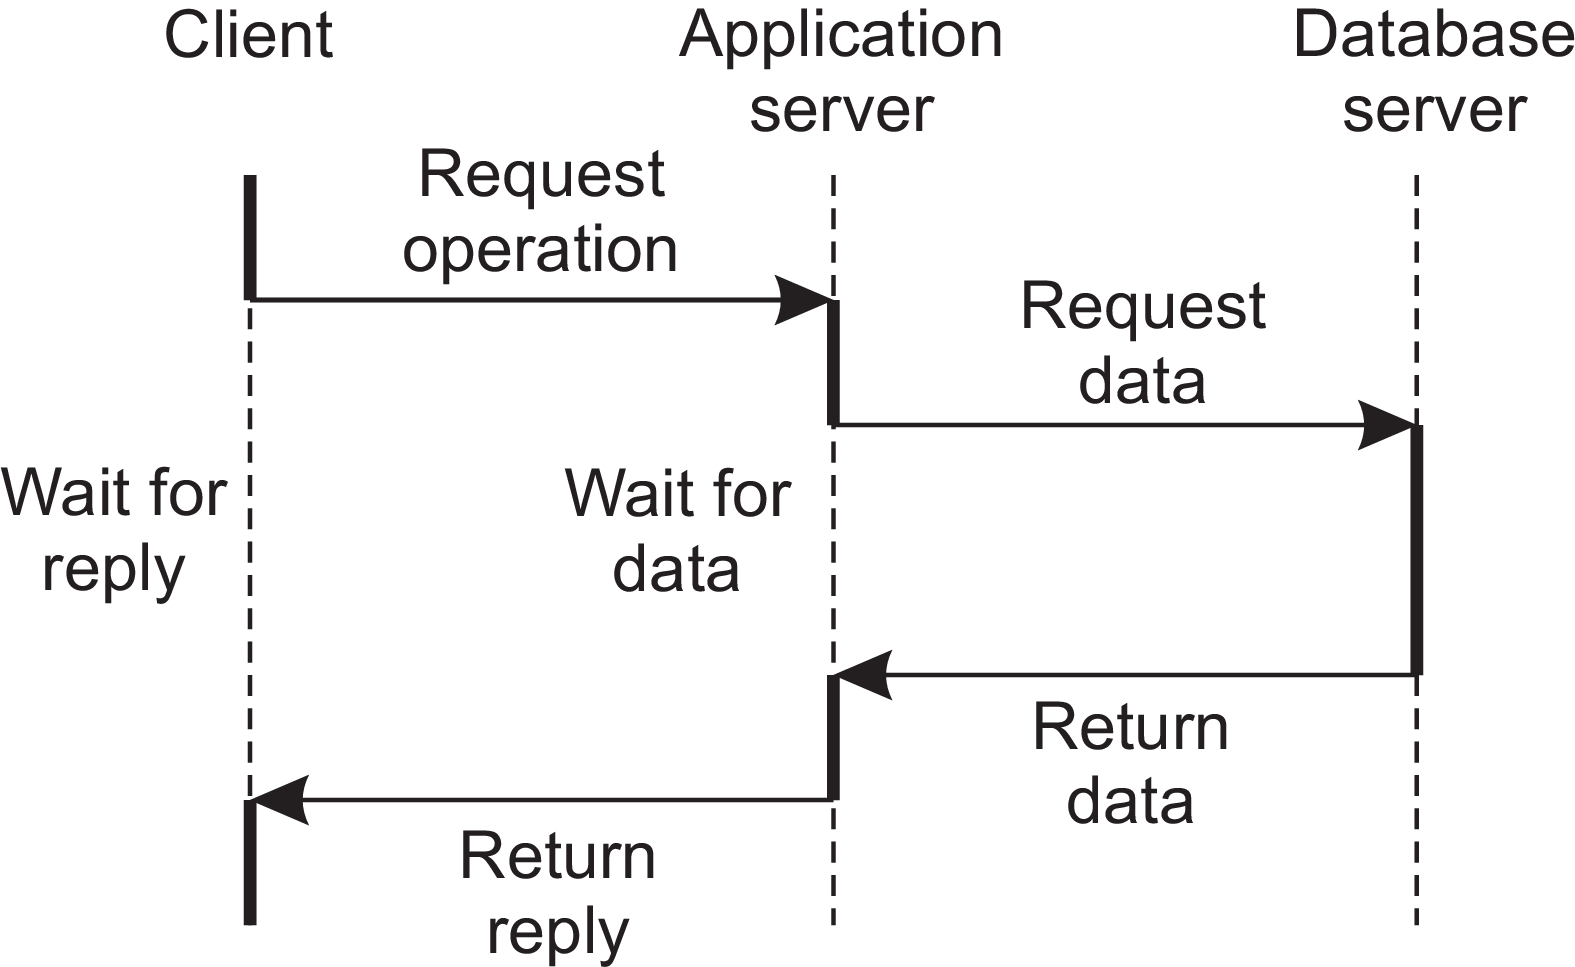
\includegraphics[width=0.75\linewidth]{images/client-server-multi.png}

\end{frame}

%% --------------------------------------------------------

\begin{frame}{Organização de arquitetura de sistema centralizada}

\vspace{1cm}

\centering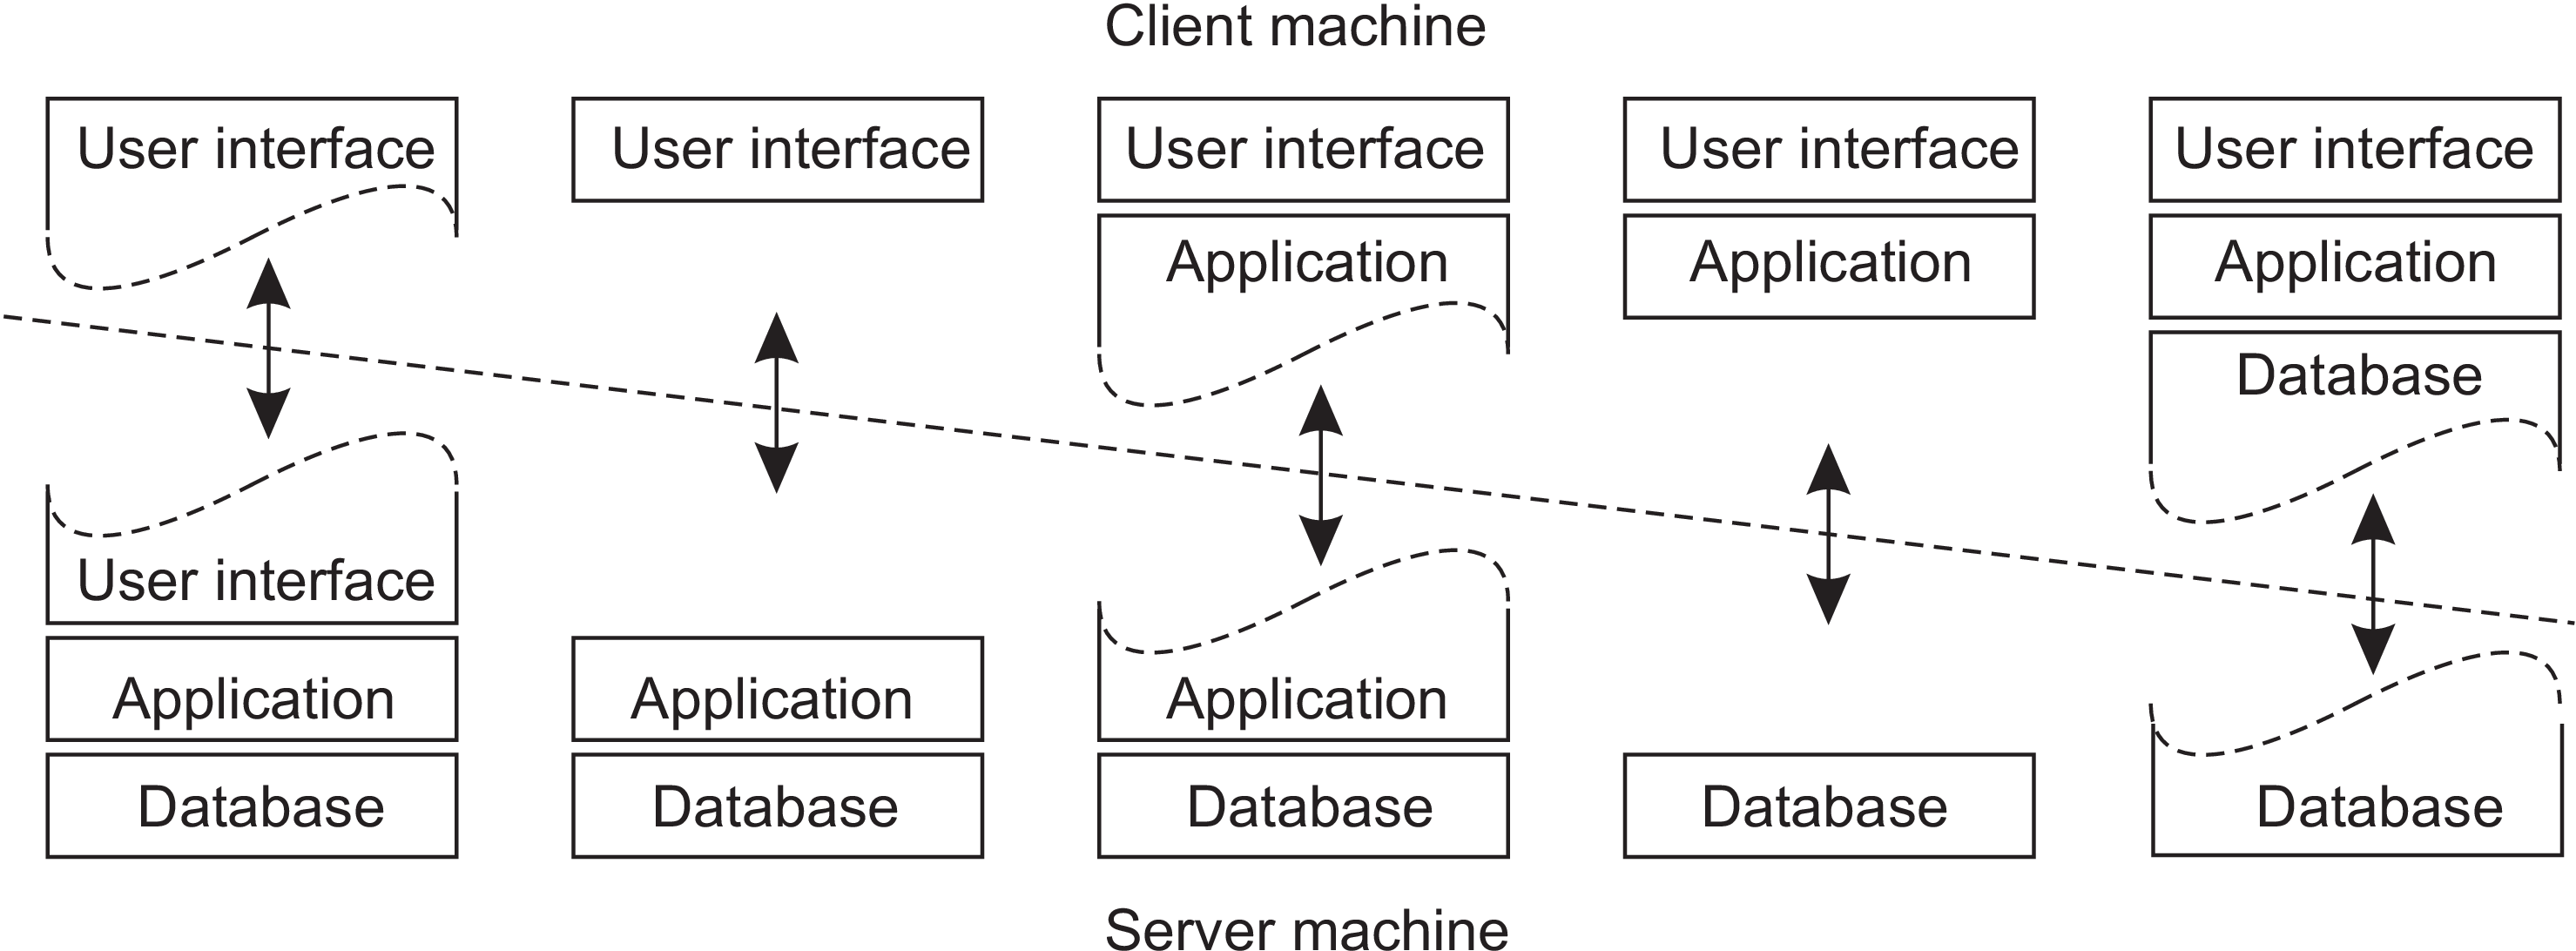
\includegraphics[width=\linewidth]{images/client-server-different.png}

\end{frame}

%% --------------------------------------------------------

\begin{frame}{Arquitetura de sistema descentralizada}

Basicamente, são as arquiteturas de sistemas Peer-to-Peer (P2P)

Neste tipo de arquitetura, dizemos que temos uma distribuição horizontal
\begin{itemize}
    \item Clientes e servidores divididos em partes
    \item Cada cliente ou servidor opera uma parte do sistema
    \begin{itemize}
        \item Uma parte dos dados, por exemplo
    \end{itemize}
    \item Balanceamento de carga
\end{itemize}
\end{frame}

%% --------------------------------------------------------

\begin{frame}{Arquitetura P2P estruturadas}

Nós são organizados em uma topologia específica
\begin{itemize}
    \item Anel
    \item Grid
    \item Árvore
    \item $\ldots$
\end{itemize}

Cada nó tem um identificador único
\begin{itemize}
    \item Um nó pode mandar mensagem para outros utilizando este identificador
    \item Tabela hash distribuída
\end{itemize}
\end{frame}

%% --------------------------------------------------------

\begin{frame}{Arquitetura P2P estruturadas}

\centering Estrutura de hipercubo

\vspace{1cm}

\centering 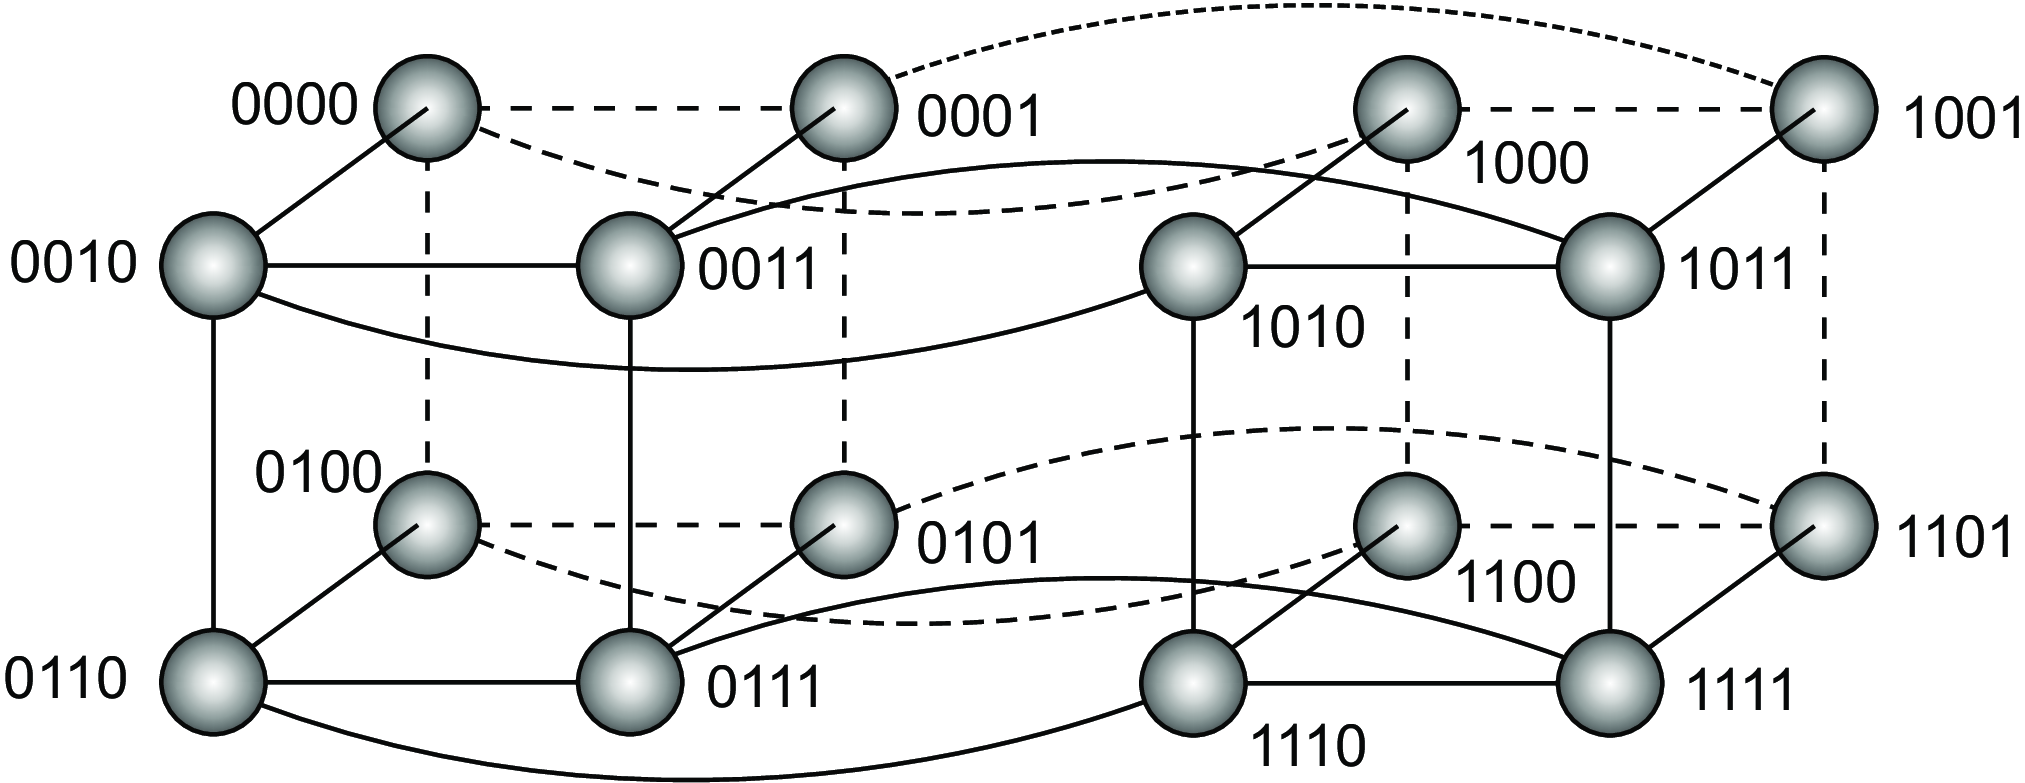
\includegraphics[width=\textwidth]{images/hypercube.png}
\end{frame}

%% --------------------------------------------------------

\begin{frame}{Arquitetura P2P não estruturadas}

Não existe uma tabela hash distribuída com o endereço dos nós do sistema

\vspace{1cm}

Ao invés disso, cada nó possui uma lista com o endereço de seus vizinhos
\begin{itemize}
    \item Tabela construida de forma \textit{ad-hoc}
    \item Tabela construída de forma dinâmica
    \begin{itemize}
        \item A tabela permite inclusões, remoções e modificações
    \end{itemize}
\end{itemize}

\end{frame}

%% --------------------------------------------------------

\begin{frame}{Arquitetura P2P não estruturadas}

Vantagens:
\begin{itemize}
    \item Fácil de incluir ou remover nós do sistema
    \begin{itemize}
        \item Escalabilidade do sistema
    \end{itemize}
\end{itemize}

\vspace{0.5cm}

Desvantagens:
\begin{itemize}
    \item Dados não podem ser localizados instantaneamente
    \begin{itemize}
        \item É necessário realizar uma busca
        \item \textit{Flooding}
        \item \textit{Random walks}
    \end{itemize}
\end{itemize}
\end{frame}

%% --------------------------------------------------------

\begin{frame}{\textit{Flooding}}

Busca em largura

\begin{enumerate}
    \item Um nó interessado em um dado faz a requisição para seus vizinhos
    \item Caso o vizinho possua a informação, ele responde
    \item Caso contrário, ele retransmite a requisição para seus vizinhos
    \begin{itemize}
        \item Caso o vizinho já tenha recebido a requisição antes, ele não retransmite mais
    \end{itemize}
\end{enumerate}

Necessário informar o tempo de vida (TTL) da mensagem
\begin{itemize}
    \item Muito curto: dado provavelmente não será encontrado
    \item Muito longo: muito caro, grande número de troca de mensagens
\end{itemize}
\end{frame}

%% --------------------------------------------------------

\begin{frame}{\textit{Random Walk}}

Busca em profundidade

\begin{enumerate}
    \item Um nó interessado em um dado faz a requisição para um de seus vizinhos, escolhido de forma aleatória
    \item Caso o vizinho possua a informação, ele responde
    \item Caso contrário, ele retransmite a requisição para outro de seus vizinhos, de forma aleatória
\end{enumerate}

Necessário informar o máximo número de retransmissões

Além disso, pode-se iniciar múltiplos \textit{random walks} em paralelo
\begin{itemize}
    \item Cada um iniciando em um vizinho diferente
\end{itemize}
\end{frame}

%% --------------------------------------------------------

\begin{frame}{Métodos de busca}

\vspace{1cm}

\centering 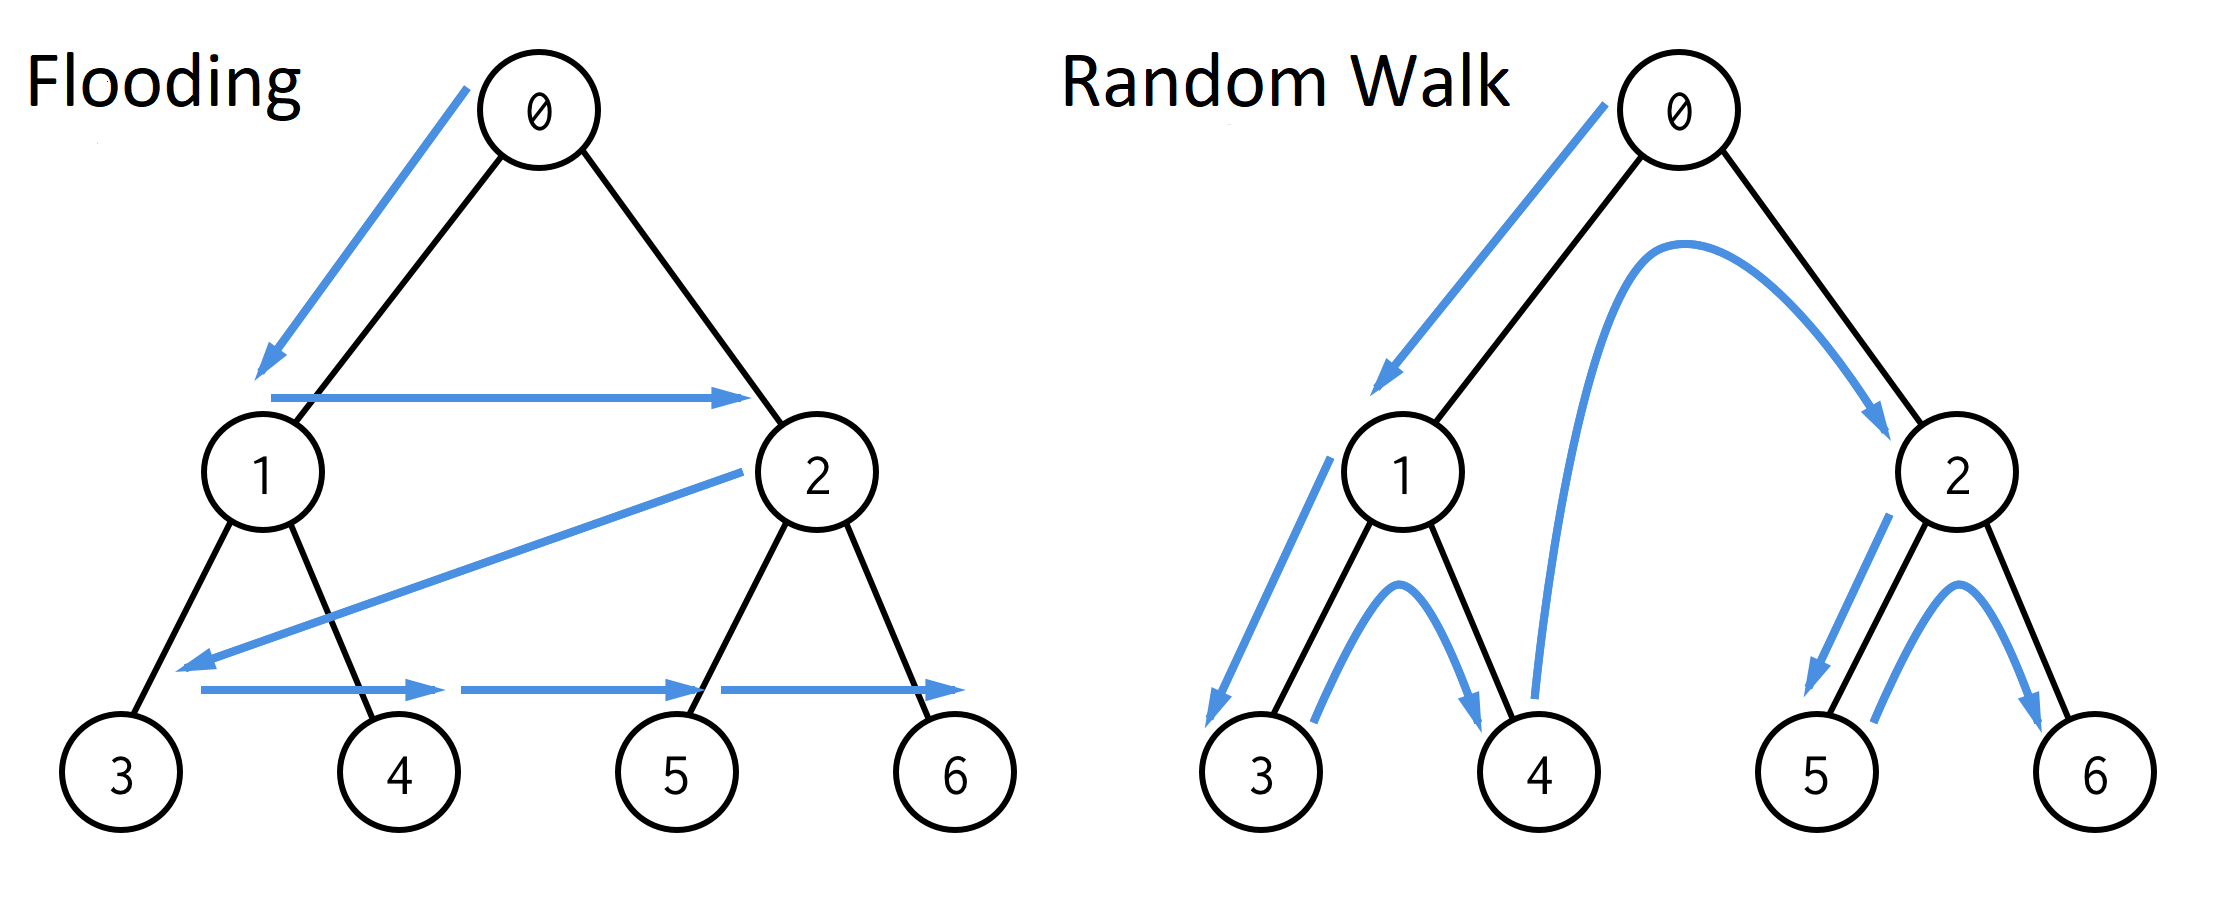
\includegraphics[width=\textwidth]{images/busca.png}
\end{frame}

%% --------------------------------------------------------

\begin{frame}{Arquitetura P2P semi-estruturada}

Construidas utilizando hierarquia de nós
\begin{itemize}
    \item Super nós
    \begin{itemize}
        \item Escolhidos através de uma eleição
        \item Devem ter alta disponibilidade
    \end{itemize}
    \item Nós fracos
    \begin{itemize}
        \item Se ligam a um super nó
    \end{itemize}
\end{itemize}

Existe uma arquitetura P2P estruturada entre os super nós

Cada super nó funciona como \textit{gateway} para uma outra rede P2P
\begin{itemize}
    \item Pode ser estruturada ou não
\end{itemize}
\end{frame}

%% --------------------------------------------------------

\begin{frame}{Arquitetura P2P semi-estruturada}

 \vspace{1cm}

\centering 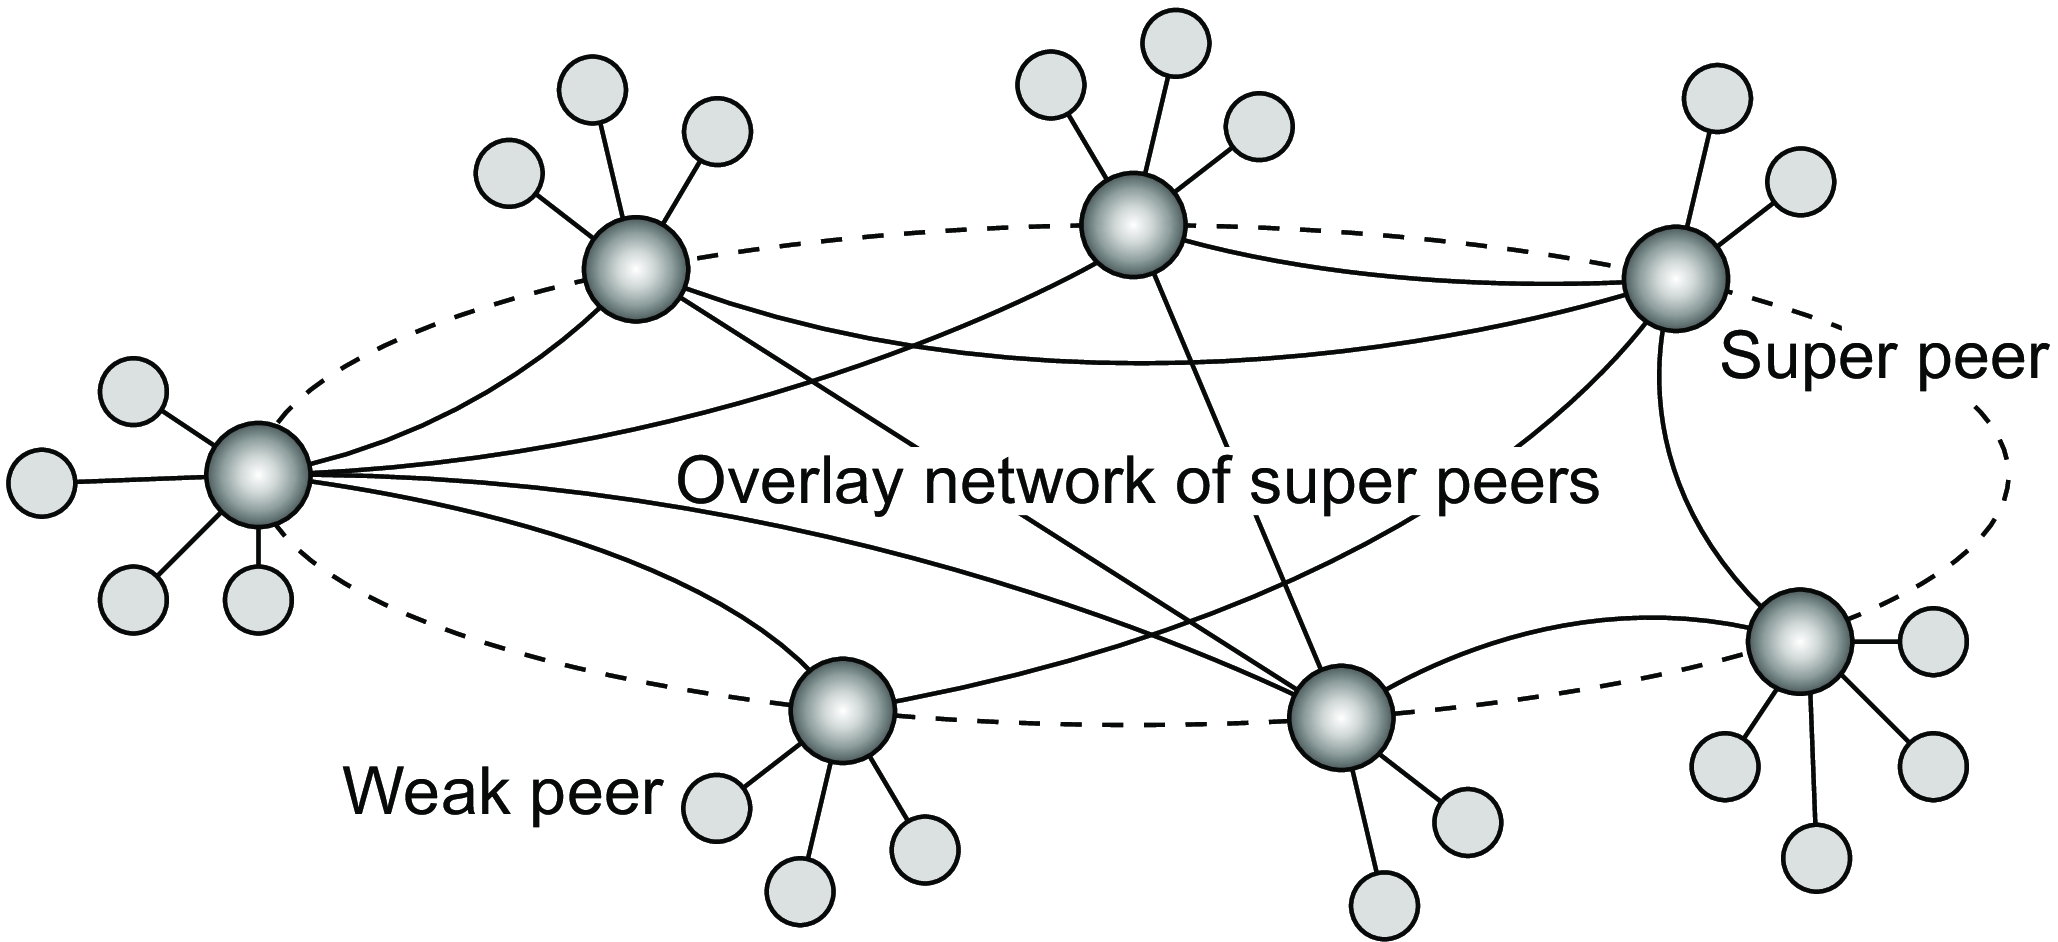
\includegraphics[width=\textwidth]{images/semi-estruturada.png}
\end{frame}

%% --------------------------------------------------------

\begin{frame}{Arquiteturas híbridas}

Combinam características das arquiteturas centralizadas e descentralizadas
\begin{itemize}
    \item BitTorrent
    \item Domain Names Service (DNS)
    \item Internet Service Providers (ISP)
\end{itemize}

Estruturas são muito mais complexas e utilizadas para construir sistemas distribuídos de larga escala
\end{frame}

\end{document}
% \begin{columns}[T]
%     \begin{column}{.45\textwidth}
%         Um processo envia uma requisição (ou arquivo, ou dado) 
        
%         \vspace{0.5cm}
        
%         Cria uma notificação avisando o que ele fez
        
%         \vspace{0.5cm}
        
%         Outros processos podem acessar
%     \end{column}
%     \begin{column}{.54\textwidth}
%         \vspace{0.78cm}
%         \centering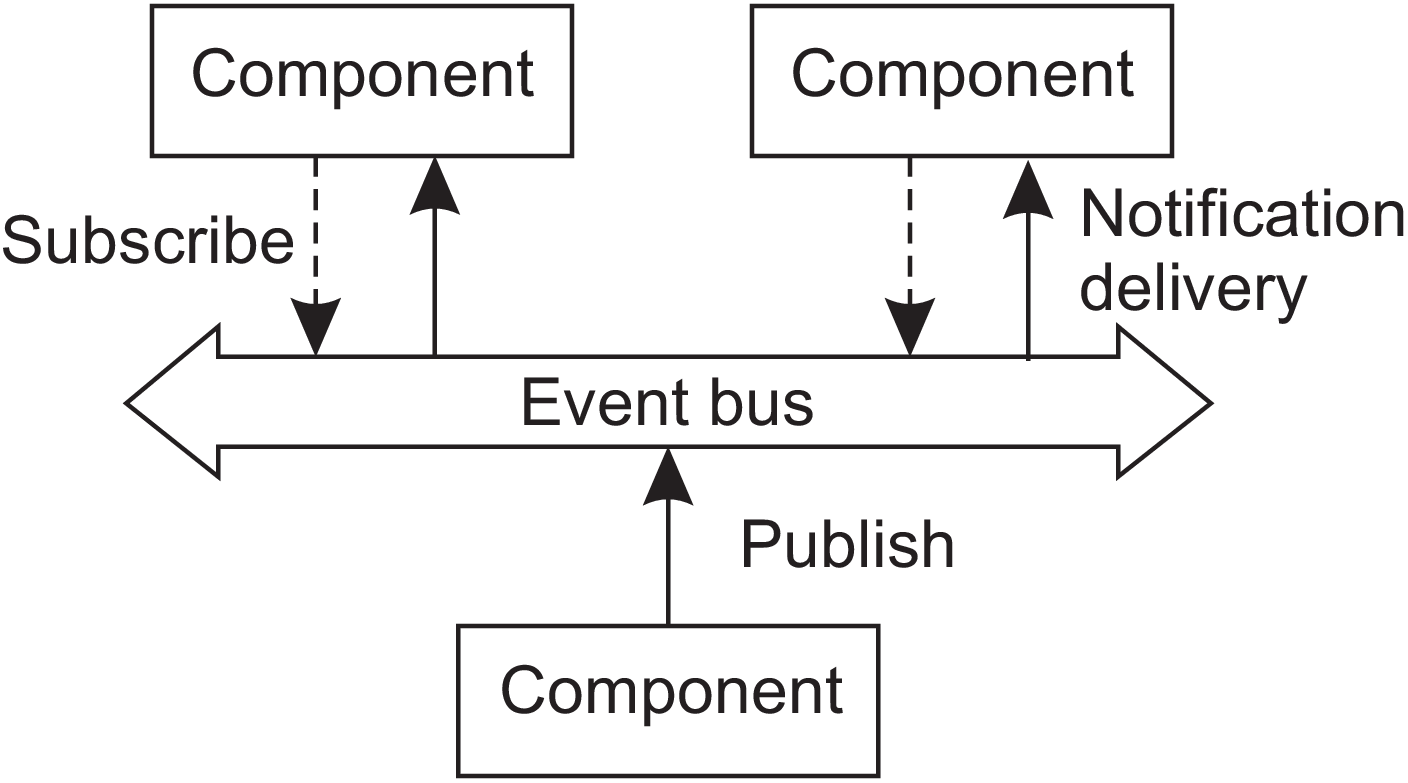
\includegraphics[width=0.95\textwidth]{images/arquitetura_eventos.png}
%     \end{column}
% \end{columns}